\documentclass[11pt]{article}
\usepackage{amsmath, amssymb, amsfonts, amsthm}
\usepackage{geometry}
\geometry{letterpaper, margin=0.5in}
\usepackage{booktabs}
\usepackage{tikz}
\usepackage{hyperref}

\newcommand{\noi}{\noindent}

\theoremstyle{definition} 
\newtheorem{definition}{Definition}[section]

\newif\ifrootsystemirreducible
\rootsystemirreducibletrue

\title{Pinned group summary: SL(n=3)}
\author{Pinning-Sympy automated output}
\date{\today}

\begin{document}

\maketitle
\tableofcontents

\newpage

\section{Basic group attributes}

\begin{tabular}{|l|l|}
	\hline
    Group & SL(n=3) \\
	\hline
    Matrix size & $3 \times 3$ \\
	\hline
    Rank & $2$ \\
	\hline
	Defining equations & $DefiningEquationPlaceholder$ \\
	\hline
\end{tabular}



\subsection{Lie algebra}

The defining equations for the Lie algebra are:
\[
LieAlgebraEquationPlaceholder
\]
A generic element of the Lie algebra is:
\[
\left[\begin{matrix}x_{0 0} & x_{0 1} & x_{0 2}\\x_{1 0} & x_{1 1} & x_{1 2}\\x_{2 0} & x_{2 1} & - x_{0 0} - x_{1 1}\end{matrix}\right]
\]

\subsection{Torus}

The torus has rank $2$. A generic element of the torus is
\[
\left[\begin{matrix}t_{0} & 0 & 0\\0 & t_{1} & 0\\0 & 0 & \frac{1}{t_{0} t_{1}}\end{matrix}\right]
\]
The rows of the matrix below are trivial characters:
\[
\left[\begin{matrix}1 & 1 & 1\end{matrix}\right]
\]

\newpage
\section{Root system}

\begin{tabular}{|l|l|}
	\hline
    Dynkin type & $A_2$ \\
	\hline
    Irreducible & True \\
	\hline
    Reduced & True \\
	\hline
	Simply laced & True \\
	\hline
	Number of roots & $6$ \\
	\hline
\end{tabular}

\subsection{Dynkin diagram}

\ifrootsystemirreducible
The root system is irreducible and has Dynkin diagram:
\else
The root system is reducible with RootSystemComponentsPlaceholder components. The Dynkin diagrams of the respective components are:
\fi

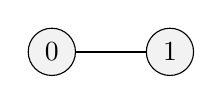
\begin{tikzpicture}[
    node/.style={circle, draw, fill=black!5, minimum size=6mm, inner sep=0pt},
    arrow/.style={-latex, thick},
    doublearrow/.style={double, double distance=2pt, -latex, thick},
    triplearrow/.style={double, double distance=4pt, -latex, thick},
    plain/.style={thick},
    baseline=(current bounding box.center)
]
    \node[node] (0) at (0.00, 0.00) {$0$};
    \node[node] (1) at (1.50, 0.00) {$1$};
    \draw[plain] (0) -- (1);
\end{tikzpicture}

\subsection{Cartan matrix}

\ifrootsystemirreducible
The root system is irreducible and has Cartan matrix:
\else
The root system is reducible with RootSystemComponentsPlaceholder components. The Cartan matrices of the respective components are:
\fi

\[
\left[\begin{matrix}2 & -1\\-1 & 2\end{matrix}\right]
\]

\subsection{Roots}

\begin{tabular}{|l|c|c|c|}
    \hline
    \textbf{Root} & \textbf{Simple} & \textbf{Sign} & \textbf{Multipliable} \\
    \hline
    $\left( -1, \  0, \  1\right)$ & No & $-$ & No \\
    \hline
    $\left( -1, \  1, \  0\right)$ & No & $-$ & No \\
    \hline
    $\left( 0, \  -1, \  1\right)$ & No & $-$ & No \\
    \hline
    $\left( 0, \  1, \  -1\right)$ & Yes & $+$ & No \\
    \hline
    $\left( 1, \  -1, \  0\right)$ & Yes & $+$ & No \\
    \hline
    $\left( 1, \  0, \  -1\right)$ & No & $+$ & No \\
    \hline
\end{tabular}


\subsection{Coroots}

\begin{tabular}{|l|l|}
    \hline
    \textbf{Root} & \textbf{Coroot} \\
    \hline
    $\left( -1, \  0, \  1\right)$ & $\left( -1, \  0, \  1\right)$ \\
    \hline
    $\left( -1, \  1, \  0\right)$ & $\left( -1, \  1, \  0\right)$ \\
    \hline
    $\left( 0, \  -1, \  1\right)$ & $\left( 0, \  -1, \  1\right)$ \\
    \hline
    $\left( 0, \  1, \  -1\right)$ & $\left( 0, \  1, \  -1\right)$ \\
    \hline
    $\left( 1, \  -1, \  0\right)$ & $\left( 1, \  -1, \  0\right)$ \\
    \hline
    $\left( 1, \  0, \  -1\right)$ & $\left( 1, \  0, \  -1\right)$ \\
    \hline
\end{tabular}


\subsection{Linear combinations of roots}

\begin{definition}
For two roots $\alpha, \beta$ in a root system $\Phi$, the set of positive integral linear combinations of $\alpha, \beta$ that are also roots is denoted
\(
	(\alpha, \beta) = \{ i \alpha + j \beta \in \Phi : i, j \in \mathbb{Z}_{\ge 1} \}
\).
\end{definition}

\begin{tabular}{|l|l|c|}
    \hline
    $\alpha$ & $\beta$ & Pairs $(i,j)$ \\
    \hline
    $\left( -1, \  0, \  1\right)$ & $\left( 0, \  1, \  -1\right)$ & $(1,1)$ \\
    \hline
    $\left( -1, \  0, \  1\right)$ & $\left( 1, \  -1, \  0\right)$ & $(1,1)$ \\
    \hline
    $\left( -1, \  1, \  0\right)$ & $\left( 0, \  -1, \  1\right)$ & $(1,1)$ \\
    \hline
    $\left( -1, \  1, \  0\right)$ & $\left( 1, \  0, \  -1\right)$ & $(1,1)$ \\
    \hline
    $\left( 0, \  -1, \  1\right)$ & $\left( 1, \  0, \  -1\right)$ & $(1,1)$ \\
    \hline
    $\left( 0, \  1, \  -1\right)$ & $\left( 1, \  -1, \  0\right)$ & $(1,1)$ \\
    \hline
\end{tabular}


\newpage
\section{Root spaces}

\subsection{Dimensions}

The table below lists each root along with the dimension of the associated root space (and root subgroup).

RootSpaceDimensionPlaceholder

\subsection{Root space table}

\noi The table below lists each root along with a generic element of the associated root space (inside the Lie algebra). Include a definition here? INCOMPLETE

RootSpaceTablePlaceholder

\newpage
\section{Root subgroups}

\subsection{Root subgroup table}

\noi The table below lists each root along with a generic element of the associated root subgroup.

RootSubgroupTablePlaceholder

\subsection{Homomorphism property}

\noi Background theoretical info on homomorphism/pseudo-homomorphism property INCOMPLETE

HomomorphismDefectTablePlaceholder

\noi Below is an explicit formulation of the homomorphism/pseudo-homomorphism identities.

HomomorphismDefectIdentitiesPlaceholder

\newpage
\section{Commutators}

\noi Background theoretical info on commutator relation INCOMPLETE

\noi Because of its relevance to commutators, we repeat here the table of linear combinations of roots.

\begin{tabular}{|l|l|c|}
    \hline
    $\alpha$ & $\beta$ & Pairs $(i,j)$ \\
    \hline
    $\left( -1, \  0, \  1\right)$ & $\left( 0, \  1, \  -1\right)$ & $(1,1)$ \\
    \hline
    $\left( -1, \  0, \  1\right)$ & $\left( 1, \  -1, \  0\right)$ & $(1,1)$ \\
    \hline
    $\left( -1, \  1, \  0\right)$ & $\left( 0, \  -1, \  1\right)$ & $(1,1)$ \\
    \hline
    $\left( -1, \  1, \  0\right)$ & $\left( 1, \  0, \  -1\right)$ & $(1,1)$ \\
    \hline
    $\left( 0, \  -1, \  1\right)$ & $\left( 1, \  0, \  -1\right)$ & $(1,1)$ \\
    \hline
    $\left( 0, \  1, \  -1\right)$ & $\left( 1, \  -1, \  0\right)$ & $(1,1)$ \\
    \hline
\end{tabular}


\subsection{Commutator coefficient table}

\noi The table below gives the coefficients $N_{ij}^{\alpha\beta}$.

CommutatorCoefficientTablePlaceholder

\subsection{Commutator identities}

\noi Below is an explicit formulation of the commutator formula identities.

CommutatorIdentitiesPlaceholder

\newpage
\section{Weyl group}

\noi Background theoretical info on Weyl group, especially as realized inside the group, including info on conjugation between root subgroups INCOMPLETE

\subsection{Weyl group elements}

\noi The table below lists roots along with an associated Weyl group element.

WeylGroupPlaceholder

\subsection{Weyl group conjugation coefficients}

\noi The table below lists roots along with the coefficients obtain in performing conjugation by an associated Weyl element.

WeylConjugationCoefficientPlaceholder

\subsection{Weyl group conjugation identities}

\noi Below is an explicit formulation of the Weyl group conjugation identities.

WeylConjugationIdentitiesPlaceholder

\end{document}